\documentclass[
	a4page,
	parskip=full,
	12pt
]{scrartcl}
\usepackage[margin=2.5cm]{geometry}
\usepackage{libertinus, libertinust1math}
\usepackage[sfdefault]{biolinum}
\usepackage{roboto}
\usepackage{amsmath,amssymb,amsfonts,amsthm}
\usepackage{graphicx, hyperref, wrapfig}
\usepackage[
	sorting=none,
	style=verbose
]{biblatex}
\addbibresource{literature.bib}


\begin{document}

{
	\sffamily\noindent
	Leon Oleschko \hfill \today\\
	Modeling Quantum Hardware: open dynamics and control \hfill Universität Konstanz\\
	\vspace*{1cm}\\
	\textbf{\huge Project Proposal}
}

Since reading the noise modelling in a proposal for a gravitation wave observatory \autocite{rainer_weiss_electronically_1972}
I want make a similar analysis of a noise limited experiment.
By examining a optomechanical resonance cavity with the numerical tools form this course, this can be achieved.

\begin{wrapfigure}{R}{3.5cm}
	\includegraphics{figures/drawing.pdf}
\end{wrapfigure}
The setup explored here is a single optomechanical cavity. 
It is schematically drawn right, with a resonant cavity and a room temperature mirror, modelled as a high $Q$ oscillator.
Then the noise sources from the temperature bath of the mirror mount, the radiation pressure noise and the shot (or phase) noise are introduced, as those are the main noise sources \autocite{aspelmeyer_cavity_2014-1}.
It should be possible to write this easily in the Lindblad framework of the course and solved using the common numerical tools.\\
The project can be extended by looking into modelling a simple squeezing implementation, to minimize the radiation pressure noise \autocite{caves_quantum-mechanical_1980,aspelmeyer_cavity_2014-1}.

\section*{Implementation}
There a 3 main frequencies: The frequency of the mechanical oscillator $\Omega$, the frequency of the optical cavity $\omega_0 - G \hat x$ depending on the mirror position $\hat x$ and the frequency of the input laser $\omega_L$. \autocite{aspelmeyer_cavity_2014-1}
One of the frequencies can be eliminated by going into a rotating frame. 
Here $\omega_L$ is chosen, and the detuning $\Delta = \omega_L - \omega_0$ is introduced.
With this the linearized Hamiltonian can be written for the simplest coupling:$$
	H_0 / \hbar = - (\Delta + G \hat x) \hat a^\dagger \hat a + \Omega \hat b^\dagger b
$$
as the sum of the energy in the optical field with $\hat a^\dagger \hat a$ photons and in the mechanical with $\hat b^\dagger \hat b$ phonons.
This can be rewritten using $\hat x = \sqrt{\hbar / 2m\Omega} \;(\hat b + \hat b^\dagger)$.


\end{document}
